\documentclass[resume]{subfiles}



\begin{document}
\section{Patterns}
\subsection{Process}
\subsubsection{6Q}
\begin{figure}[H]
\centering
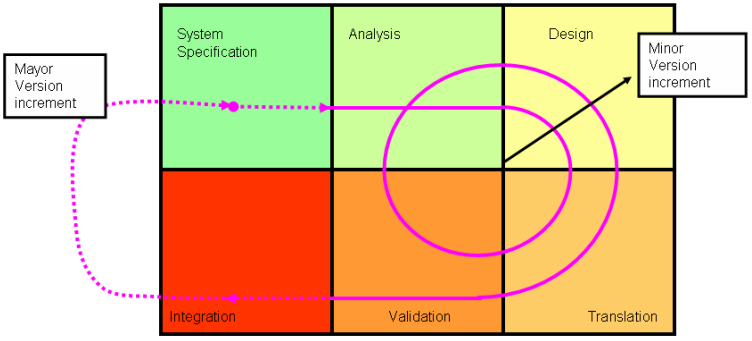
\includegraphics[width=7.00cm]{img_3.png}
\end{figure}
\subsection{Factory}
\begin{figure}[H]
\centering
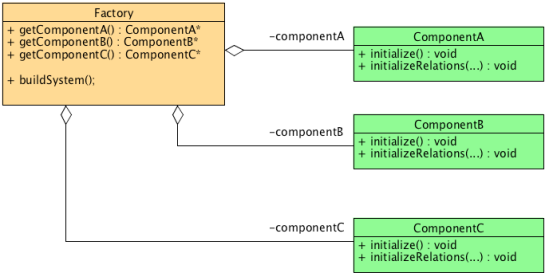
\includegraphics[width=7.00cm]{img_4.png}
\end{figure}
\begin{enumerate}
\item \verb!create!
\item \verb!initialize!
\item \verb!initializeRelations! quand tous les \verb!create! et \verb!initialize! sont faits
\end{enumerate}
\subsection{Observateur}
\begin{figure}[H]
\centering
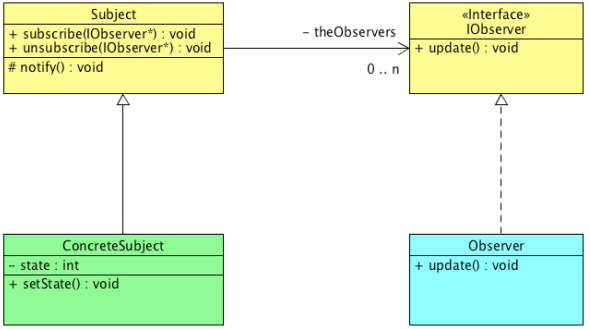
\includegraphics[width=7.00cm]{img_5.png}
\end{figure}
\subsection{Interface}
\begin{figure}[H]
\centering
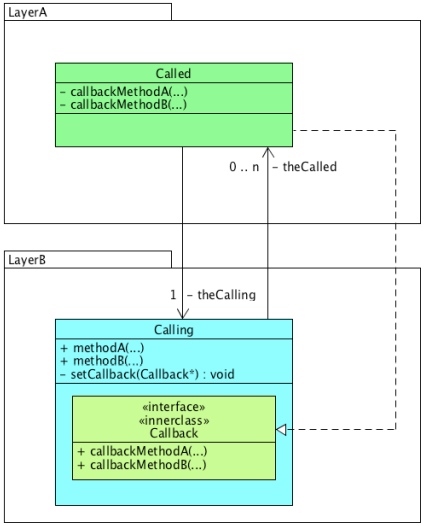
\includegraphics[width=7.00cm]{img_6.png}
\end{figure}
\begin{figure}[H]
\centering
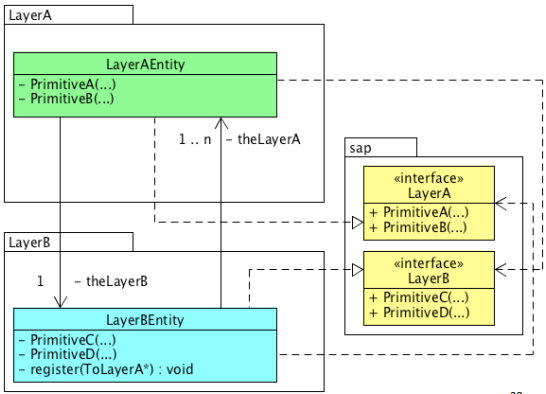
\includegraphics[width=7.00cm]{img_7.png}
\end{figure}






\end{document}